%\documentclass[aspectratio=169]{beamer}
\documentclass[10pt,aspectratio=169,xcolor={table,dvipsnames}]{beamer}
\usefonttheme[onlymath]{serif}
\usepackage{animate}


\mode<presentation>
{
  \usetheme{Madrid}      % or try Darmstadt, Madrid, Warsaw, ...
  \usecolortheme{dolphin} % or try albatross, beaver, crane, ...
  \usefonttheme{default}  % or try serif, structurebold, ...
  \setbeamertemplate{navigation symbols}{}
  \setbeamertemplate{caption}[numbered]
  \setbeamertemplate{headline}{}
}

\documentclass[a4paper,12pt]{report}
\usepackage[english]{babel}
\usepackage[left=2cm,right=2cm,top=2cm,bottom=2cm]{geometry}
%\usepackage{mathtools}
\usepackage{amsthm}     % for definitions and theorems
\usepackage[many]{tcolorbox}    % boxes around definitions and theorems
%\usepackage{amsmath}
%\usepackage{nccmath}
\usepackage{amssymb}    % \ltimes
\usepackage{etoolbox}   % for start of Chapter
%\usepackage{amsfonts}
\usepackage{physics}    % for all Physics related
\usepackage{dsfont}     % for the identity matrix symbol \1
%\usepackage{mathrsfs}

\usepackage{titling}
\usepackage{indentfirst}

\usepackage{bm}
\usepackage[dvipsnames]{xcolor}
\usepackage{cancel}

\usepackage{xurl}
\usepackage[colorlinks=true]{hyperref}

\usepackage{float}
\usepackage{graphicx}
\usepackage{subcaption}
%\usepackage{tikz}

\usepackage{ctable}     % tabelas
\renewcommand{\P}{\phantom{+}}  % empty space to indent things
\usepackage{multirow}
\usepackage{tabulary}

%%%%%%%%%%%%%%%%%%%%%%%%%%%%%%%%%%%%%%%%%%%%%%%%%%%

\newcommand{\eps}{\epsilon}
\newcommand{\vphi}{\varphi}
\newcommand{\cte}{\text{cte}}

\newcommand{\N}{{\mathbb{N}}}
\newcommand{\Z}{{\mathbb{Z}}}
%\newcommand{\Q}{{\mathbb{Q}}}
\newcommand{\C}{{\mathbb{C}}}
\renewcommand{\S}{{\hat{S}}}
%\renewcommand{\H}{\s{H}}

\renewcommand{\a}{{\vb{a}}}
\renewcommand{\b}{{\vb{b}}}
\renewcommand{\d}{{\dagger}}
\newcommand{\up}{{\uparrow}}
\newcommand{\down}{{\downarrow}}
\newcommand{\hc}{{\text{h.c.}}}

\newcommand{\ihat}{\bm{\hat{\imath}}}
\newcommand{\jhat}{\bm{\hat{\jmath}}}
\newcommand{\khat}{\bm{\hat{k}}}

\newcommand{\0}{{\vb{0}}}
\newcommand{\1}{\mathds{1}}
\newcommand{\E}{{\vb{E}}}
\newcommand{\B}{{\vb{B}}}
\renewcommand{\u}{{\vb{u}}}
\renewcommand{\v}{{\vb{v}}}
\renewcommand{\r}{{\vb{r}}}
\newcommand{\R}{{\vb{R}}}
\newcommand{\Q}{{\vb{Q}}}
\newcommand{\G}{{\vb{G}}}
\newcommand{\g}{{\vb{g}}}
\renewcommand{\k}{{\vb{k}}}
\newcommand{\K}{{\vb{K}}}
\newcommand{\p}{{\vb{p}}}
\newcommand{\q}{{\vb{q}}}
\newcommand{\F}{{\vb{F}}}
\renewcommand{\t}{{\vb{t}}}
\newcommand{\vtau}{{\bm{\tau}}}
\newcommand{\vdelta}{{\bm{\delta}}}

% COLORED SYMMETRY ELEMENTS
\newcommand{\Ct}{{\textcolor{Cyan}{C_3}}}
\newcommand{\Ctn}[1]{{\textcolor{Cyan}{C_3^{\textcolor{black}{#1}}}}}
\newcommand{\Cs}{{\textcolor{ForestGreen}{C_6}}}
\newcommand{\Csn}[1]{{\textcolor{ForestGreen}{C_6^{\textcolor{black}{#1}}}}}
\newcommand{\sd}{{\textcolor{RoyalBlue}{\sigma_d}}}
\newcommand{\sdn}[1]{{\textcolor{RoyalBlue}{\sigma_d^{\textcolor{black}{#1}}}}}
\newcommand{\sdp}{{\textcolor{RoyalBlue}{\sigma_d'}}}
\newcommand{\sdpp}{{\textcolor{RoyalBlue}{\sigma_d''}}}
\newcommand{\sv}{{\textcolor{Orange}{\sigma_v}}}
\newcommand{\svn}[1]{{\textcolor{Orange}{\sigma_v^{\textcolor{black}{#1}}}}}
\newcommand{\svp}{{\textcolor{Orange}{\sigma_v'}}}
\newcommand{\svpp}{{\textcolor{Orange}{\sigma_v''}}}

\newcommand{\s}{\sigma}
%\newcommand{\prodint}[2]{\left\langle #1 , #2 \right\rangle}
\newcommand{\cc}[1]{\overline{#1}}
\newcommand{\Eval}[3]{\eval{\left( #1 \right)}_{#2}^{#3}}
\newcommand{\sg}[2]{\{ #1 \mid #2 \}}

\newcommand{\unit}[1]{\; \mathrm{#1}}

\newcommand{\n}{\medskip}
\newcommand{\e}{\quad \mathrm{and} \quad}
\newcommand{\ou}{\quad \mathrm{or} \quad}
\newcommand{\virg}{\, , \;}
\newcommand{\ptodo}{\forall \,}
\renewcommand{\implies}{\; \Rightarrow \;}
%\newcommand{\eqname}[1]{\tag*{#1}} % Tag equation with name

\setlength{\droptitle}{-7em}

\makeatletter
\patchcmd{\chapter}{\if@openright\cleardoublepage\else\clearpage\fi}{}{}{}  % start 'Chapter' at the same page. needs package etoolbox
\makeatother

%% Theorems, definitions, proofs
\theoremstyle{definition}

\newtheorem{definition}{Definition}[section]
\tcolorboxenvironment{definition}{
  colback=blue!5!white,
  boxrule=0pt,
  boxsep=1pt,
  left=2pt,right=2pt,top=2pt,bottom=2pt,
  oversize=2pt,
  sharp corners,
  before skip=\topsep,
  after skip=\topsep,
}

\newtheorem{theorem}{Theorem}[section]
\tcolorboxenvironment{theorem}{
  colback=blue!5!white,
  boxrule=0pt,
  boxsep=1pt,
  left=2pt,right=2pt,top=2pt,bottom=2pt,
  oversize=2pt,
  sharp corners,
  before skip=\topsep,
  after skip=\topsep,
}


%%%%%%%%%%%%%%%%%%%%%%%%%%%%%%%%%%%%%%%%%%%%%%%%%%%%%%%%%

\title[Topological Quantum Chemistry]{\LARGE{Topological Quantum Chemistry}}
\author[Mateus Marques]{
\large{Mateus Marques
}}
\date{\today}

\begin{document}

\begin{frame}
  \titlepage
\end{frame}


\begin{frame}

There are two standard approaches to study the properties of crystals \cite{tms17}:

\n

\begin{itemize}
\item Chemists usually prefer solving the Schrödinger equation in real space, for example by DFT. They emphasize the concepts of orbitals.
\item For the other hand, physicists prefer to work on reciprocal space, where the Hamiltonian is block diagonal and the description is given in terms of energy bands $E(\k)$.
\end{itemize}

The goal of Topological Quantum Chemistry (TQC) is to link these two descriptions through the concept of band representation (BR). Zak \cite{zak1981} realized that BRs can be decomposed into what he called ``elementary band representations'' (EBRs), i.e., a class of BRs that cannot be further decomposed.
\begin{figure}[H]
\centering
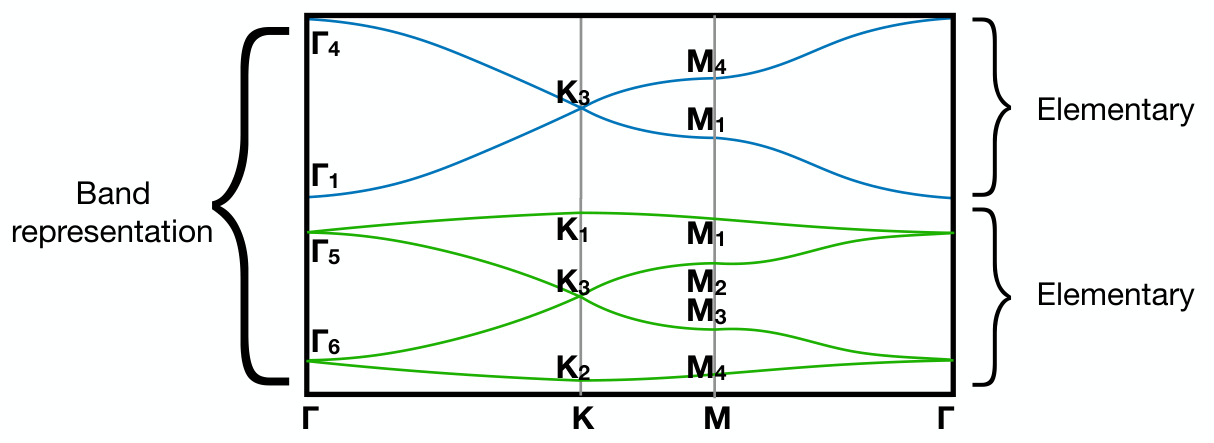
\includegraphics[width=0.7\linewidth]{fig/ebrs.png}
\end{figure}


\end{frame}

\begin{frame}
We will follow the development of the theory with the hexagonal lattice (monolayer graphene) example in mind.
\begin{figure}[H]
\centering
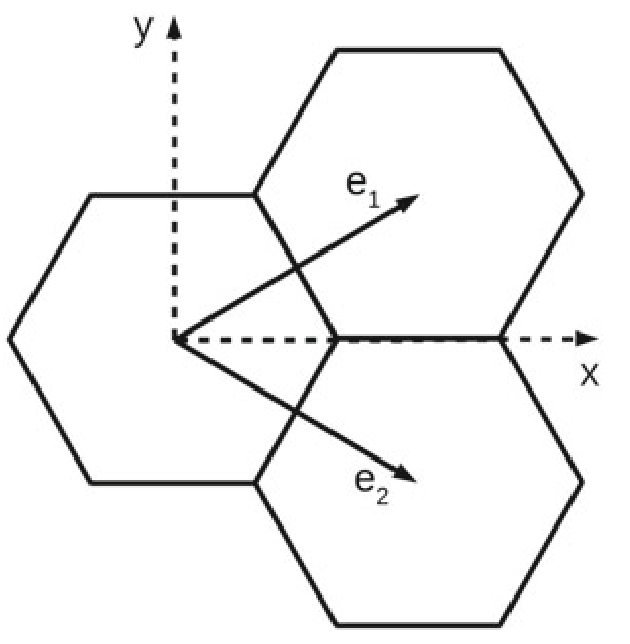
\includegraphics[width=0.25\linewidth]{fig/hexagonal_frame.png}
\end{figure}

The Bravais lattice vectors in our convention are
$$
\vb{e}_1 = \frac{\sqrt{3}}{2} \vu{x} + \frac{1}{2} \vu{y}
$$
$$
\vb{e}_2 = \frac{\sqrt{3}}{2} \vu{x} - \frac{1}{2} \vu{y}
$$
\end{frame}

\begin{frame}
There are:
\begin{itemize}
\item 32 point groups, and 230 space groups in 3D.
\item 10 point groups, and 17 space groups in 2D (wallpaper groups).
\end{itemize}

The 2D hexagonal lattice corresponds to wallpaper group \#17, or the corresponding space group $P6mm$ (\#183). It is a symmorphic space group, and its point group generators can be chosen as
\begin{equation*}
\vcenter{\hbox{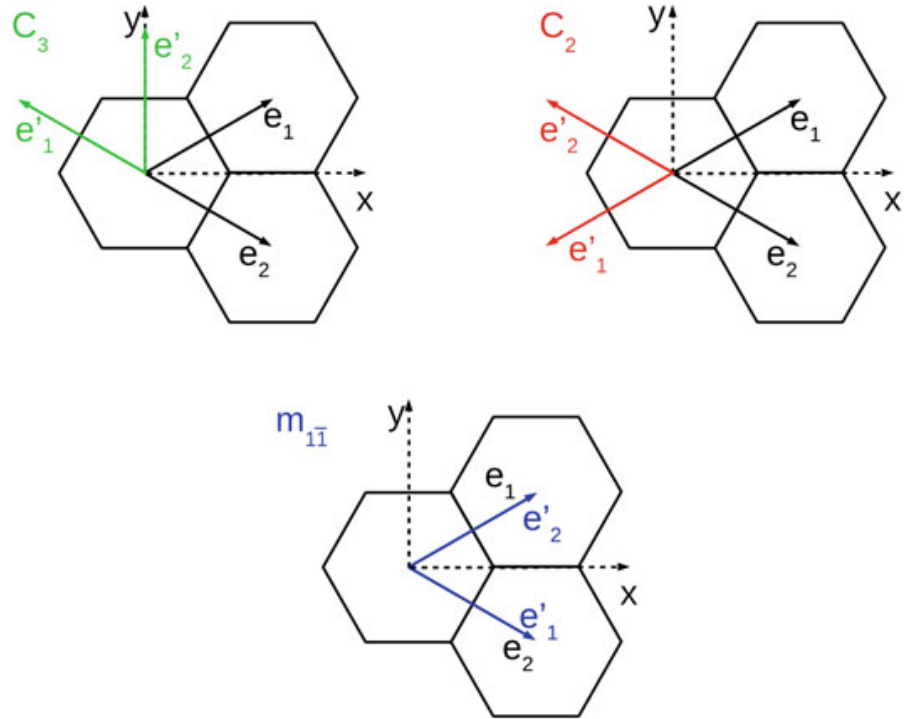
\includegraphics[width=0.38\linewidth]{fig/hexagonal_generators.png}}}
\qquad\qquad
\begin{aligned}
C_3: (\vb{e}_1, \vb{e}_2) \to (-\vb{e}_2, \vb{e}_1 - \vb{e_2})
\\
C_2: (\vb{e}_1, \vb{e}_2) \to (-\vb{e}_1, -\vb{e_2})
\\
m_{1\cc{1}}: (\vb{e}_1, \vb{e}_2) \to (\vb{e}_2, \vb{e}_1)
\end{aligned}
\end{equation*}

\end{frame}

\begin{frame}
\begin{definition}[Orbit of $\q$]
It is the set of all positions related to $\q$ by elements of the space group $G$, i.e. $\text{Orb}_\q = \{g \q \mid g \in G\}$, \textit{and} belong to the same unit cell.
\end{definition}

\begin{definition}[Site-symmetry group / Stabilizer group]
The site-symmetry group of a position $\q$ is the subgroup of operations $g \in G$ that leave $\q$ fixed.
$$
G_\q = \{g \mid g \q = \q\} \leq G.
$$
\end{definition}

\textit{Remarks:}
\begin{itemize}
\item $G_\q$ can include elements $\{R \mid \r\}$, with nonzero translations, $\r \neq \0$.
\item Since any site-symmetry group leaves a point invariant, it is also isomorphic to one of the 32 crystallographic points groups (in 3D).
\end{itemize}
\end{frame}

\begin{frame}
\begin{definition}[Wyckoff position]
A \textit{Wyckoff position} $\q$ is any position in the unit cell of the crystal. There are \textit{special} Wyckoff positions, which are those which are left invariant by some symmetry operations. The \textit{multiplicity} of a Wyckoff positions is the number of elements in its orbit (in the same unit cell).
\end{definition}

\begin{definition}[Coset representatives]
The \textit{coset representatives} of site-symmetry group are the elements that generate the orbit of Wyckoff position. The number of coset representatives is also equal to the multiplicity of the Wyckoff position.
\end{definition}

\begin{definition}[Coset decomposition]
Given a Wyckoff position $\q$, the \textit{coset decomposition} with respect to $\q$ is the full space group is defined by
$$
G = \bigcup_\alpha g_\alpha (G_{\q} \ltimes \Z^d).
$$
\end{definition}
\end{frame}

\begin{frame}{Site-symmetry groups}
\begin{figure}[H]
\centering
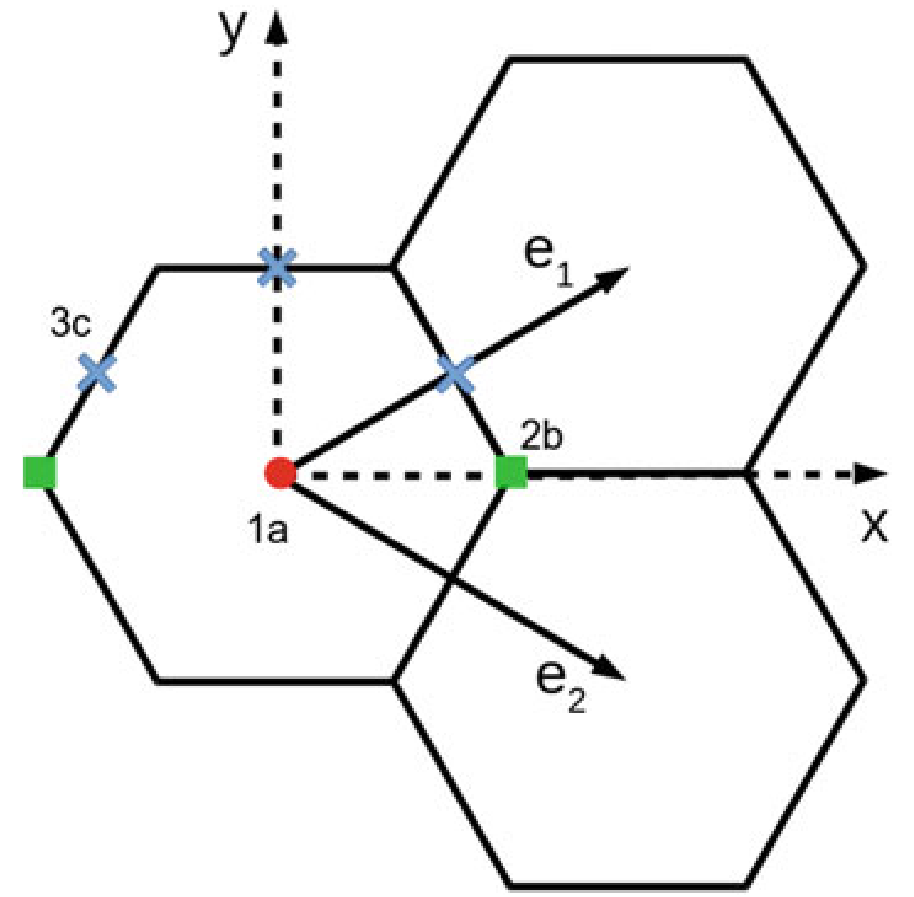
\includegraphics[width=0.22\linewidth]{fig/wyckoff_pos.png}
\end{figure}
\begin{itemize}
\item $\q = (\e_1 - \e_2) / 2 = \e_y / 2$ (\textcolor{blue}{blue cross}). Site-symmetry group $\simeq C_{2v}$ or $D_2$.
\begin{align*}
\sg{m_{11}}{0}: (\e_1, \e_2) \to (-\e_2, -\e_1)
\\
\q = \frac{\e_1-\e_2}{2} \to \frac{\e_1-\e_2}{2} = \q
\end{align*}
\begin{align*}
\sg{C_2}{1\cc{1}}: [(\e_1, \e_2) \to (-\e_1, -\e_2)] + (\e_1 - \e_2)
\\
\q = \frac{\e_1-\e_2}{2} \to \qty[\frac{-\e_1+\e_2}{2}] + (\e_1 - \e_2) = \q
\end{align*}
\end{itemize}
\end{frame}

\begin{frame}{Site-symmetry groups}
\begin{figure}[H]
\centering
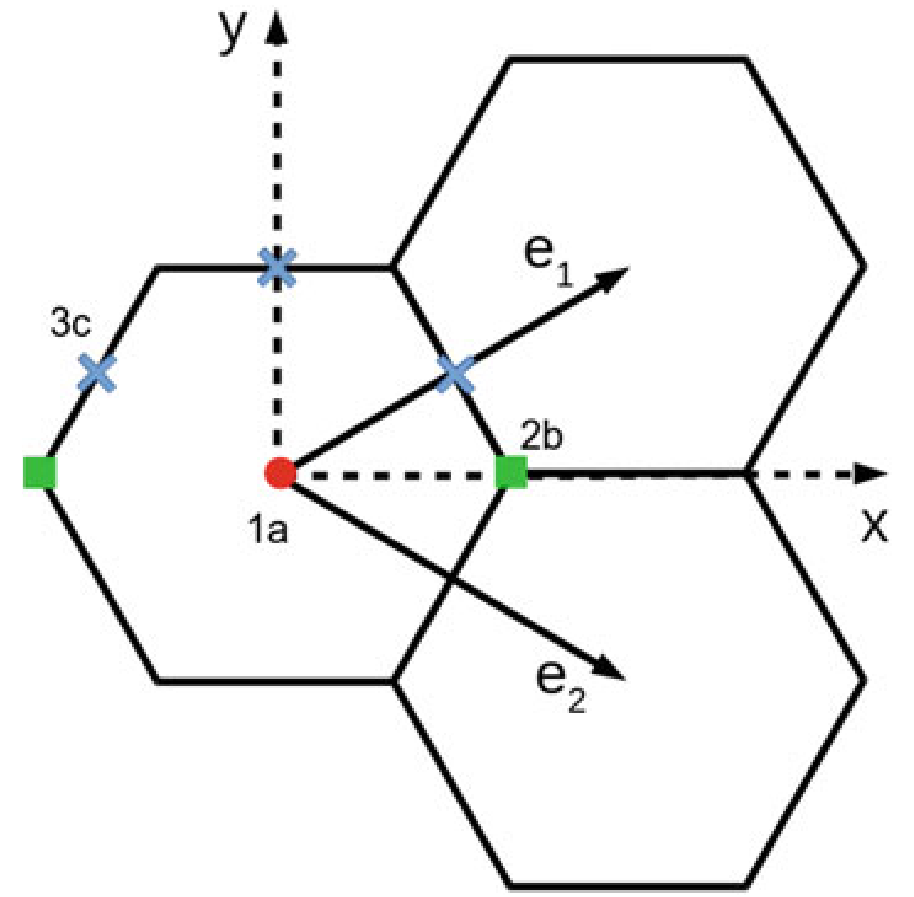
\includegraphics[width=0.22\linewidth]{fig/wyckoff_pos.png}
\end{figure}
\begin{itemize}
\item $\q = (\e_1 + \e_2) / 3$ (\textcolor{green}{green square}). Site-symmetry group isomorphic to $C_{3v}$ or $D_3$.
\begin{align*}
\sg{m_{1\cc{1}}}{0}: (\e_1, \e_2) \to (\e_2, \e_1)
\\
\q = \frac{\e_1+\e_2}{3} \to \frac{\e_2+\e_1}{3} = \q
\end{align*}
\begin{align*}
\sg{C_3}{01}: [(\e_1, \e_2) \to (-\e_2, \e_1-\e_2)] + (\e_2)
\\
\q = \frac{\e_1-\e_2}{2} \to \qty[\frac{-\e_2+(\e_1-\e_2)}{3}] + (\e_2) = \q
\end{align*}
\end{itemize}
\end{frame}

\begin{frame}{Site-symmetry groups}
\begin{figure}[H]
\centering
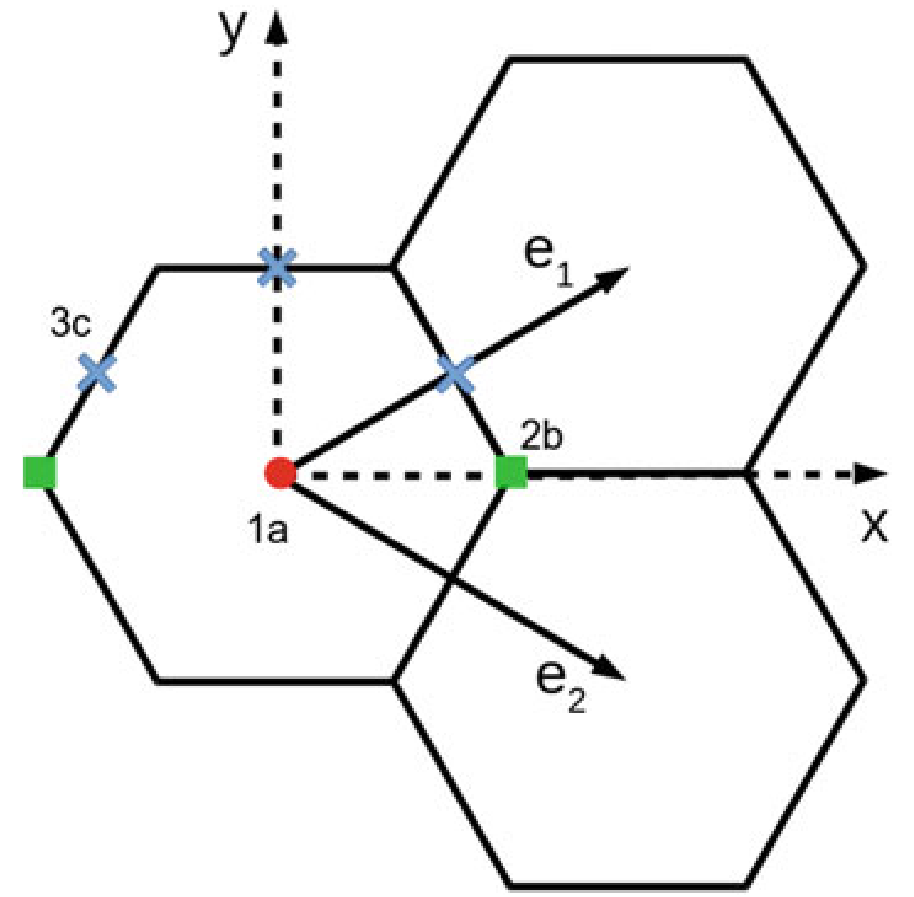
\includegraphics[width=0.22\linewidth]{fig/wyckoff_pos.png}
\end{figure}
\begin{itemize}
\item $\q = \0$ (\textcolor{red}{red dot}). Site-symmetry group isomorphic to $C_{6v}$ or $D_6$.

In this case, all elements in the point group leave this point invariant, and the stabilizer group at $\q=\0$ is not only isomorphic to the point group $C_{6v}$ of the space group, but coincides with it.

\n

\item $\q = x(\e_1+\e_2)$, $x \in \qty(0, \frac{1}{3})$ (line connecting the red dot and the green square).

In this case, we consider the line that goes from the origin to one of the vertices of the hexagon. This set of points is left unchanged by the mirror plane $m_{1\cc{1}}$. Isomorphic to $C_{1v}$.
\end{itemize}
\end{frame}

\begin{frame}{Orbits}
\begin{figure}[H]
\centering
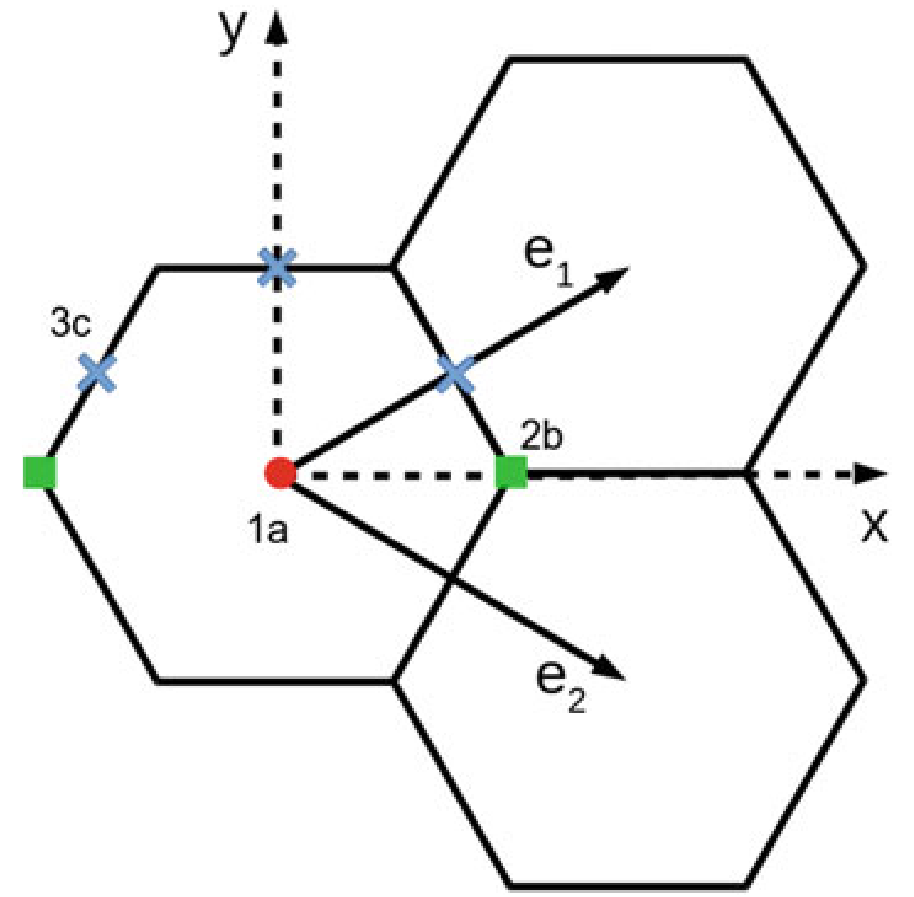
\includegraphics[width=0.22\linewidth]{fig/wyckoff_pos.png}
\end{figure}

\begin{itemize}
\item $\q = (\e_1-\e_2)/2 = \e_y/2$ (\textcolor{blue}{blue cross}).
\end{itemize}

Since the site-symmetry group for this point contains as generators the mirror plane and the 2-axis, we will use the 3-axis to generate the orbit:
\begin{align*}
\sg{C_3}{0} \qty(\frac{1}{2},-\frac{1}{2}) &= \qty(-\frac{1}{2},0)
\\
\sg{C_3^{-1}}{0} \qty(\frac{1}{2},-\frac{1}{2}) &= \qty(0,\frac{1}{2})
\end{align*}
So the orbit of q is composed by 3 points. We call these the 3c Wyckoff positions.
\end{frame}


\begin{frame}{Orbits}
\begin{figure}[H]
\centering
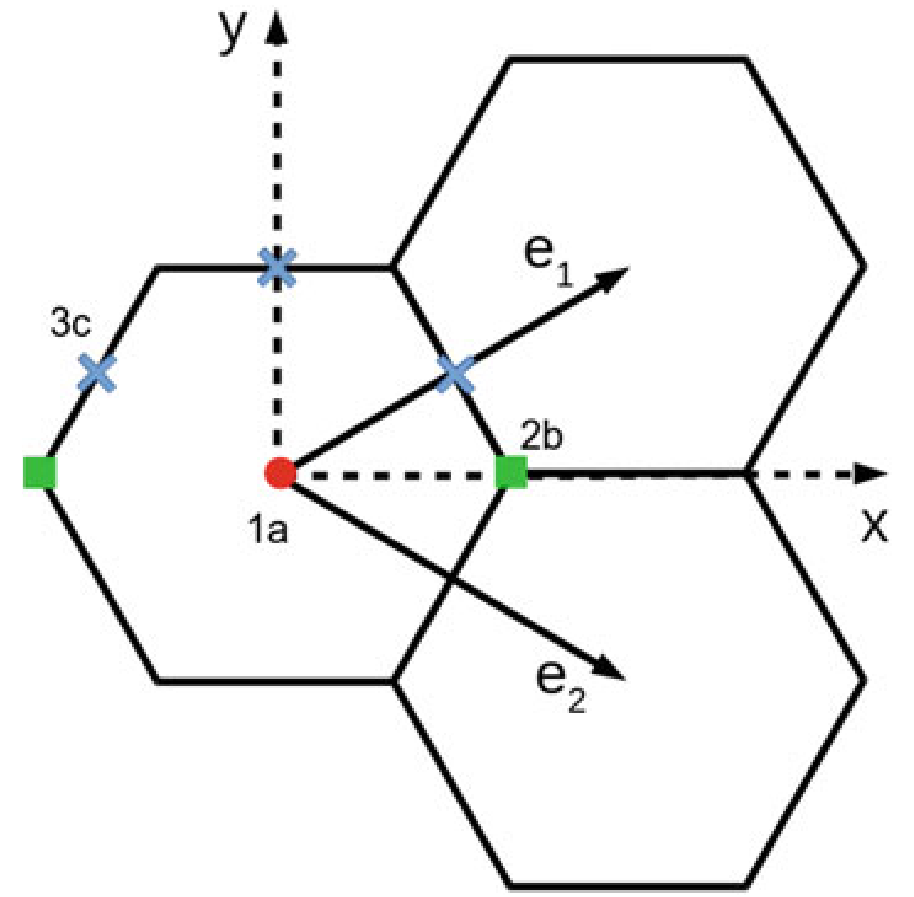
\includegraphics[width=0.22\linewidth]{fig/wyckoff_pos.png}
\end{figure}

\begin{itemize}
\item $\q = (\e_1 + \e_2) / 3$ (\textcolor{green}{green square}).

In this case, the site-symmetry group contains the mirror plane and the 3-axis, so we need to consider the 2-axis:
\begin{align*}
\sg{C_3}{0} \qty(\frac{1}{2},-\frac{1}{2}) &= \qty(-\frac{1}{2},0)
\\
\sg{C_3^{-1}}{0} \qty(\frac{1}{2},-\frac{1}{2}) &= \qty(0,\frac{1}{2})
\end{align*}
These positions are labeled as 2b Wyckoff positions.
\end{itemize}
\end{frame}


\begin{frame}{Orbits}
\begin{figure}[H]
\centering
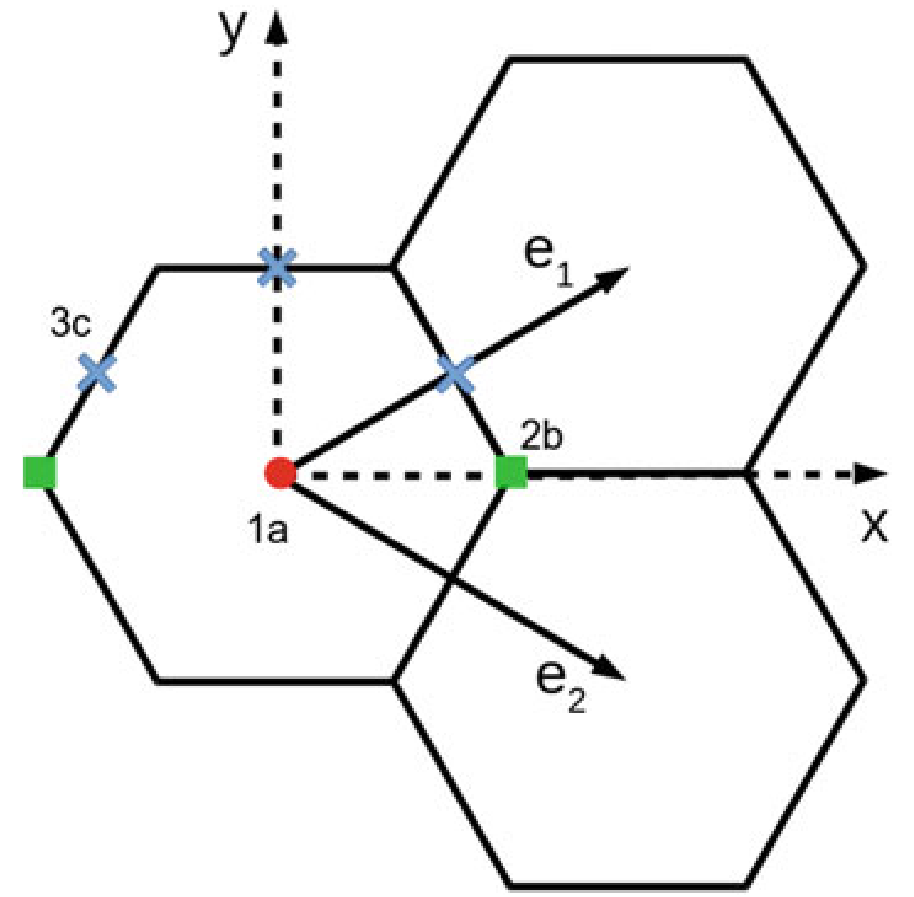
\includegraphics[width=0.22\linewidth]{fig/wyckoff_pos.png}
\end{figure}

\begin{itemize}
\item $\q = \0$ (\textcolor{red}{red dot}).

Since the site-symmetry group at this point is the whole point group, there are no other positions in its orbit. This position is denoted as 1a.

\n

\item $\q = x(\e_1+\e_2)$, $x \in \qty(0, \frac{1}{3})$ (line connecting the red dot and the green square).

The site-symmetry group for this set of points contains just the mirror plane, so any combination of the axes (the 2- and 3-axis) will generate a position in the orbit. In this case, there will be 6 positions in the orbit, which coincide with the ones generated by the 6-axis.
\end{itemize}
\end{frame}

\begin{frame}

We are interested only in orbitals that are localized at \textit{maximal Wyckoff positions}. This is because later on we will see that only the maximal ones can give rise to elementary band representations (though not necessarily).

\begin{definition}
A Wyckoff position $\q$ is said to be \textit{non-maximal} if there exists a group $H$ ($G_\q \neq H \neq G)$ such that $G_\q \subseteq H \subseteq G$. A Wyckoff position that is not non-maximal is \textit{maximal}.
\end{definition}

\n

We know that the positions for the different elements in the same orbit are related to each other by
$$
\q_\alpha = g_\alpha \q
$$
for some $\q$ in the orbit and $g_\alpha$ a coset representative. Thus, for some $h \in G_\q$,
$$
h\q = \q \implies (g_\alpha h g_\alpha^{-1}) \q_\alpha = \q_\alpha
$$
and we see that $g_\alpha h g_\alpha^{-1} \in G_{\q_\alpha}$. This is the \textit{conjugate group} $g_\alpha G_\q g_\alpha^{-1}$.
\end{frame}

\begin{frame}

$C_{6v}$ has only 3 maximal subgroups, $C_{6v}$, $C_{3v}$, and $C_{2v}$.

The maximal Wyckoff positions will be the ones whose site-symmetry group is isomorphic to one of these.

The site-symmetry groups for the positions 1a, 2b, and 3c are isomorphic to the maximal subgroups of $C_{6v}$.

The position $x (\e_1 + \e_2)$, $x \in \qty(0, 1/3)$ is not a maximal Wyckoff position, since its site-symmetry group is not maximal, e.g. $C_{1v} \subset C_{2v}, C_{3v} \subset C_{6v}$.

\n

Considering monolayer graphene, we can add $p_z$ orbitals at Wyckoff position 2b for the spinless case, or add $p_x, p_y$ orbitals at Wyckoff position 2b for the spinful case.

If the centers of charge are not localized at the atoms, but in between them, we would need to consider orbitals at Wyckoff position 3c for example.

\n

\begin{minipage}{0.32\textwidth}
\begin{figure}[H]
\centering
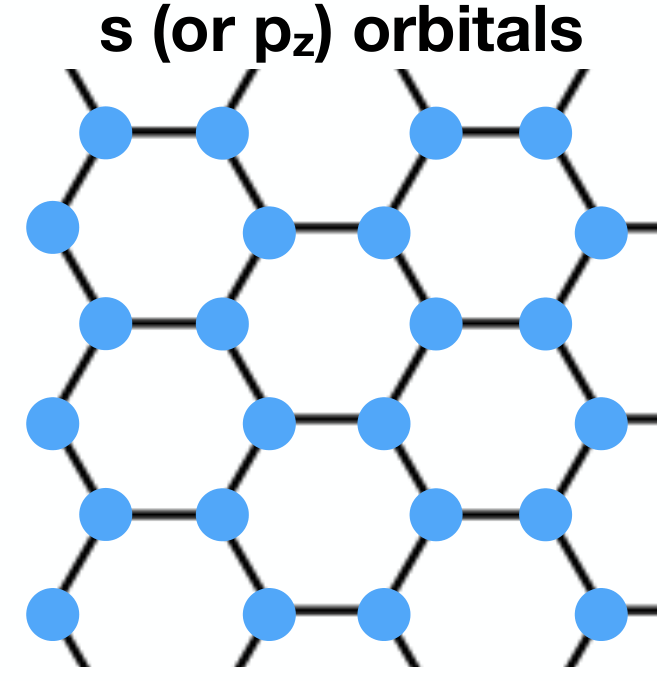
\includegraphics[height=0.5\linewidth]{fig/orbitals_pz.png}
\end{figure}
\end{minipage}
\begin{minipage}{0.32\textwidth}
\begin{figure}[H]
\centering
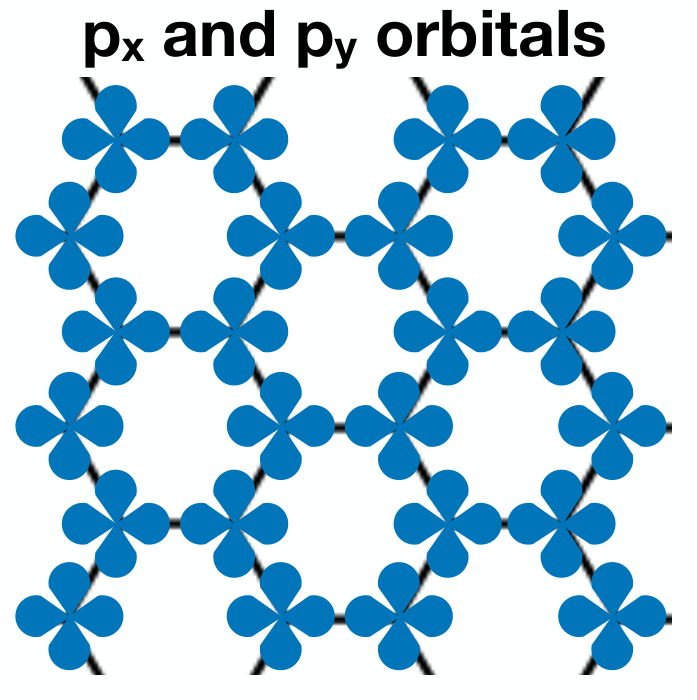
\includegraphics[height=0.5\linewidth]{fig/orbitals_pxpy.png}
\end{figure}
\end{minipage}
\begin{minipage}{0.32\textwidth}
\begin{figure}[H]
\centering
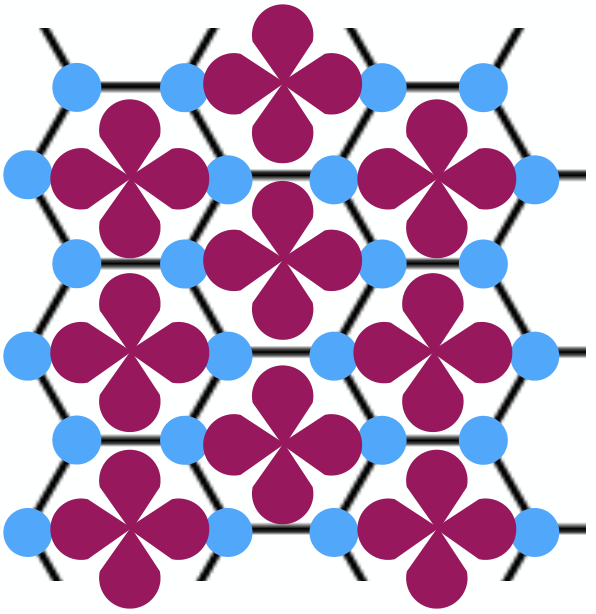
\includegraphics[height=0.5\linewidth]{fig/orbitals_strange.png}
\end{figure}
\end{minipage}

\end{frame}



\begin{frame}

\begin{definition}[Representation]
A \textit{representation} $\Pi$ of a group $G$ on a vector space $V$ is a group homomorphism $\Pi: G \to GL(V)$.
\end{definition}

\begin{definition}[Invariant subspace]
A subspace $W \subseteq V$ is said to be \textit{invariant} under a representation $\Pi$ if $\Pi(g) W \subseteq W$, for every $g \in G$.
\end{definition}

\begin{definition}[Irreducible representation]
A representation $\Pi: G \to GL(V)$ always has the (trivial) invariant subspaces $\{0\}$ and $V$. If there are not others, $\Pi$ is said to be \textit{irreducible}.
\end{definition}

\begin{theorem}[Schur's lemma]
Let $\Pi_1$ and $\Pi_2$ be two irreducible representations of $G$ in non-trivial vector spaces $V_1$, $V_2$. If $A: V_1 \to V_2$ is such that $A \Pi_1(g) = \Pi_2(g) A$ for every $g \in G$, then $A$ is bijective or $A = 0$.
\end{theorem}

\begin{theorem}[Connection with commuting operator]
Let $\mathcal{H}$ be a complex Hilbert space and $\pi: G \to GL(\mathcal{H})$ be an irreducible representation. If $A: \mathcal{H} \to \mathcal{H}$ is a bounded linear operator such that $A \pi(g) = \pi(g) A$, $\ptodo g \in G$, then $A = \lambda \cdot 1$ for some $\lambda \in \C$.
\end{theorem}

\end{frame}

\begin{frame}
\begin{enumerate}
\item
Given a (finite dimensional) Hilbert space $\mathcal{H}$ and a hamiltonian $H: \mathcal{H} \to \mathcal{H}$, we know that we can decompose the Hilbert space as
$$
\mathcal{H} = \bigoplus_{i=1}^n \mathcal{H}_i,
$$
where $H \psi = E_i \psi$, for every $\psi \in \mathcal{H}_i$. Each $\mathcal{H}_i$ is an eigenspace of $H$ associated to an eigenvalue $E_i$.

\n\n\n\n\n

\item
On the other hand, every representation $\Pi: G \to GL(\mathcal{H})$ has a decomposition
$$
\Pi = \bigoplus_{j=1}^m \pi_j, \quad \mathcal{H} = \bigoplus_{j=1}^m V_j,
$$
where $V_j \subseteq \mathcal{H}$ are invariant subspaces under $\Pi$, where $\pi_j$ are the restrictions defined by $\pi_j(g) = \eval{\Pi(g)}_{V_j}: V_j \to V_j$, which form irreducible representations $\pi_j: G \to GL(V_j)$.
\end{enumerate}

\end{frame}

\begin{frame}

What is the connection between \circled{1} and \circled{2}?

Well, if it happens that
$$
\Pi(g) H = H \Pi(g),
$$
then we can make some calculations.

\textcolor{red}{, taking the irreducible representation $\pi = \pi_j: G \to GL(V_j)$ and $A = \eval{H}_{V_j}: V_j \to V_j$<++>}

\end{frame}
<++>

%%%%%%%%%%%%%%%%%%%%%%%%%%%%%%%%%%%%%%%%%%%%%%%%%%%%%%%%%%%%%%%%%%%%%%%%%%%%%%%%

\begin{frame}
    \frametitle{References}
    \bibliographystyle{ieeetr}
    \bibliography{bibliografia}
\end{frame}

\end{document}
